\documentclass[aspectratio=169]{beamer}
\graphicspath{ {./images/}}
\usepackage{setspace}
\usepackage{hyperref}

\title{CP Rate My Professor}
\usetheme[]{Berlin}
\setbeamertemplate{navigation symbols}{}
\makeatletter
  \setbeamertemplate{footline}{%
    \begin{beamercolorbox}[colsep=1.5pt]{upper separation line foot}
    \end{beamercolorbox}
    \begin{beamercolorbox}[ht=2.5ex,dp=1.125ex,%
      leftskip=.3cm,rightskip=.3cm plus1fil]{author in head/foot}%
      \leavevmode{\usebeamerfont{author in head/foot}\insertshortauthor}%
      \hfill%
      {\usebeamerfont{institute in head/foot}\usebeamercolor[fg]{institute in head/foot}\insertshortinstitute}%
    \end{beamercolorbox}%
    \begin{beamercolorbox}[ht=2.5ex,dp=1.125ex,%
      leftskip=.3cm,rightskip=.3cm plus1fil]{title in head/foot}%
      {\usebeamerfont{title in head/foot}\insertshorttitle\hfill\insertframenumber}%
    \end{beamercolorbox}%
    \begin{beamercolorbox}[colsep=1.5pt]{lower separation line foot}
    \end{beamercolorbox}
  }
\makeatletter

\begin{document}
\section{Introduction}
\frame{\titlepage}
\begin{frame}
    \frametitle{Online Learning}
    \centering
    
\includegraphics[scale=0.5]{online_learning.jpg}
\end{frame}
\begin{frame}
    \centering
    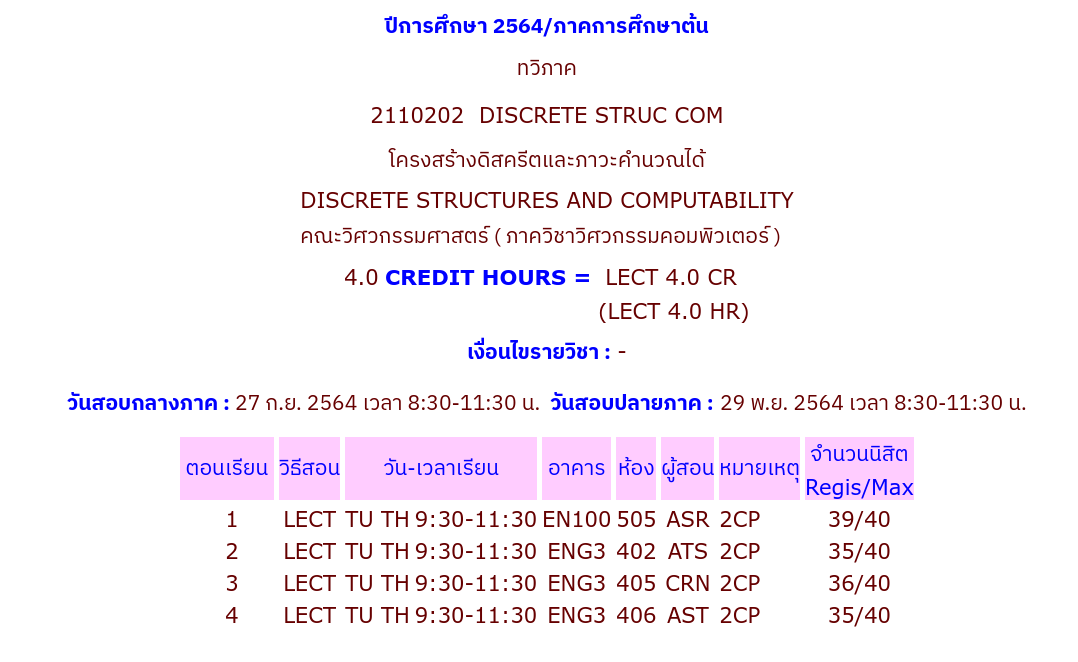
\includegraphics[scale=0.4]{discrete_section.png}
\end{frame}
\begin{frame}
    \frametitle{A sad, true story}
    \pause
    \begin{columns}
        \begin{column}{0.4\textwidth}
            \centering
            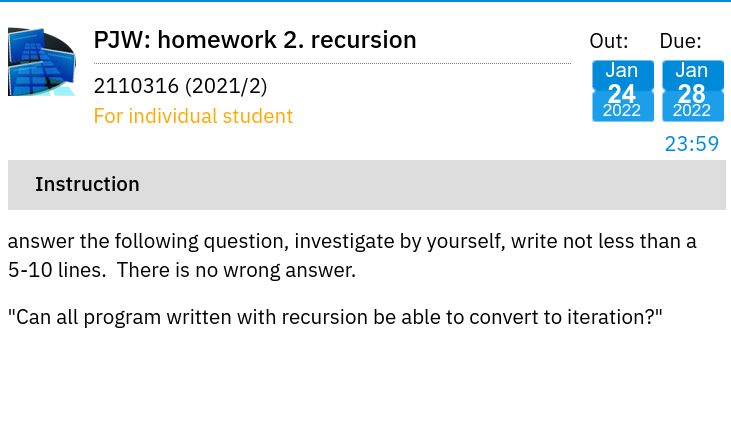
\includegraphics[scale=0.3]{proglangsec1}
            
\includegraphics[scale=0.5]{proglangsec1_nowrong}
        \end{column}
        \pause
        \begin{column}{0.4\textwidth}
            \centering
            
\includegraphics[scale=0.2]{proglangsec2}
        \end{column}
    \end{columns}
\end{frame}
\section{Application}
\begin{frame}
    \centering
    \begin{spacing}{3}
        {\huge \textbf{Meet} }\pause\\
        {\huge \color{cyan}\textbf{CP Rate My Professor}}
    \end{spacing}
\end{frame}
\begin{frame}
    \frametitle{CP Rate My Professor}
    \begin{itemize}
        \item CP Rate My Professor is a platform for commenting and rating professor\pause
    \end{itemize}
    \centering
    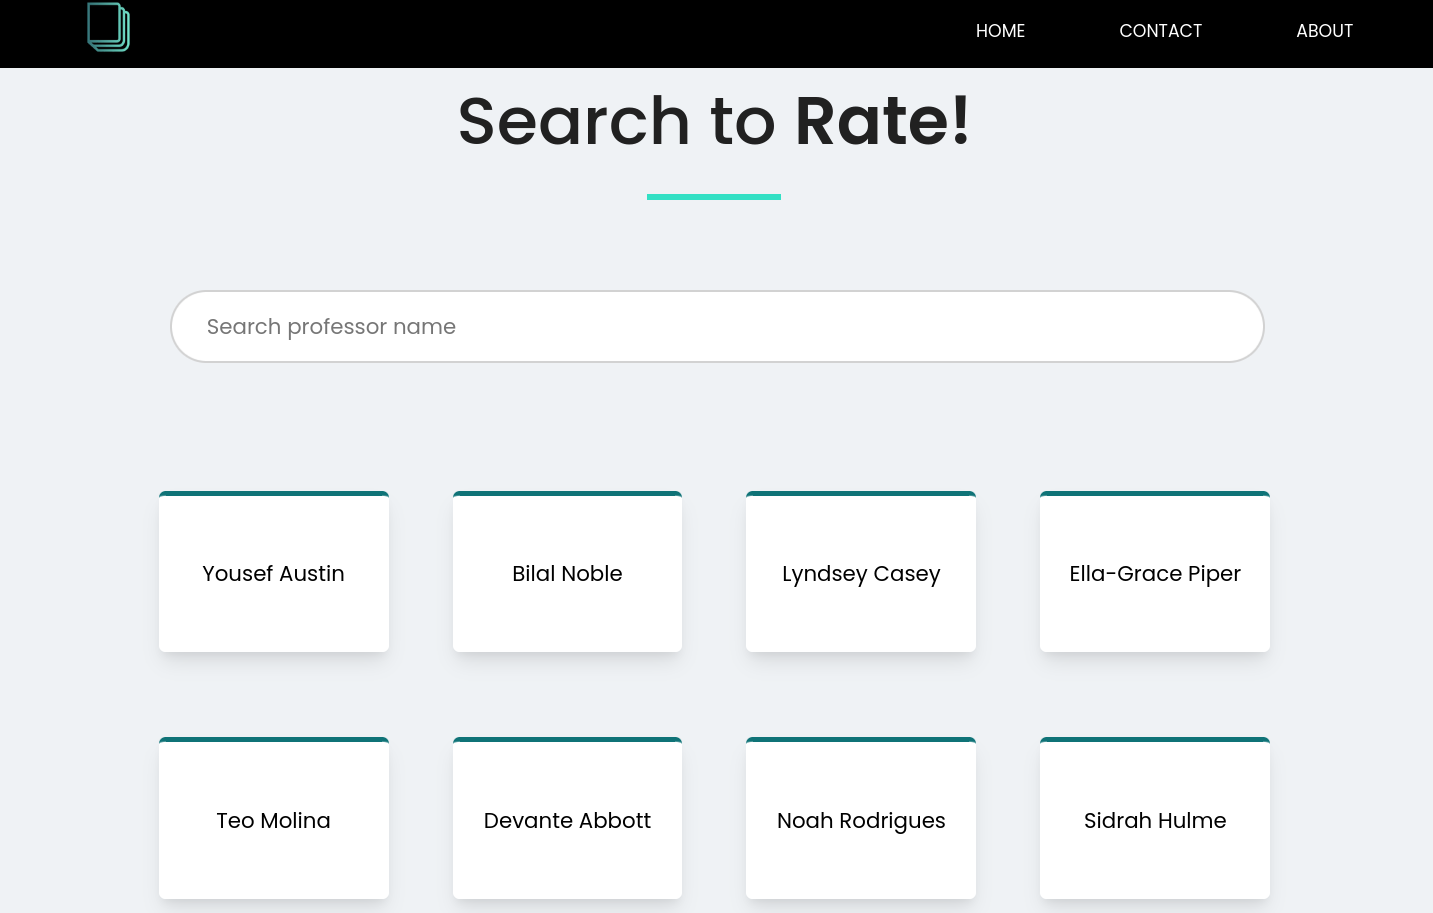
\includegraphics[scale=0.25]{ratemyprof_home.png}
\end{frame}
\begin{frame}
    \frametitle{The application}
    \begin{center}
        \begin{columns}
            \begin{column}{0.3\textwidth}
                \centering
                -- Home Page --
            \end{column}
            \begin{column}{0.3\textwidth}
                \centering
                -- Professor Page --

            \end{column}
            \centering
            -- New Comment Page --
            \begin{column}{0.3\textwidth}

            \end{column}
        \end{columns}
    \end{center}
\end{frame}
\section{Demonstration}
\begin{frame}
    \frametitle{Demonstration}
    \centering
        {\huge\textbf{Let's see the site}}\\~\\
        See the site together with us at \\
        {\color{blue}\url{https://cp-rate-my-professor.web.app}}
\end{frame}
\section{Goals}
\begin{frame}
    \frametitle{Goals}
    \begin{spacing}{1.5}
        \begin{itemize}
            \item {\color{blue}\textbf{Transparency}} and {\color{blue}\textbf{Anonymity}}
                  \begin{itemize}
                      \item We do not track our users
                      \item We only keep information that is in the comment only
                      \item User does \textbf{not} require to login to make a comment
                  \end{itemize}
            \item Be a safe space for giving comments and ratings
        \end{itemize}
    \end{spacing}
\end{frame}
\begin{frame}
    \frametitle{Important details when using the application}
    \begin{itemize}
        \item We do not allow the deletion of comment
        \item Contact information can be found at the contact page
        \item If we have information that can be proven to be false we will put the information with the comment
    \end{itemize}
\end{frame}
\begin{frame}
    \centering
    \huge{\textbf{Thank You!}}
\end{frame}
\end{document}